\documentclass[aspectratio=169]{beamer}

\usepackage[utf8]{inputenc}
\usepackage[english,russian]{babel}

\usepackage{graphicx}
\graphicspath{ {./../img/} }

\usetheme{SaintPetersburg}

%Information to be included in the title page:
\title{Самоорганизующаяся карта Кохонена}
\author{Козырев С. А.}
\institute{СПбГУ}
\date{\today}
\titlegraphic{
\includegraphics[width=0.15\linewidth]{../img/spbu_grey.eps}}

\begin{document}

\frame{\titlepage}

\begin{frame}
  \frametitle{История}
  \begin{itemize}
    \item Эту нейронную сеть предложил финский профессор Теуво Кохонен в 1980-х годах.
    \item Она основана на биологических моделях нейронных систем 1970-х годов.
  \end{itemize}
\end{frame}

\begin{frame}
  \frametitle{Нейронные сети Кохонена}
  \begin{itemize}
    \item Более широкий класс нейронных сетей, основным элементом которых является слой
    Кохонена.
    \item Слой Кохонена состоит из адаптивных линейных сумматоров («линейных
    формальных нейронов»).
    \[
      y_{j}=w_{{j0}}+\sum _{{i=1}}^{m}w_{{ji}}x_{i},
    \]
    где:
    \begin{itemize}
      \setlength\itemsep{0em}
      \item $w_{{ji}}$ — весовой коэффициент $i$-го входа $j$-го нейрона;
      \item $i$ — номер входа;
      \item $j$ — номер нейрона;
      \item $w_{{j0}}$ — пороговый коэффициент.
    \end{itemize}
    \item Как правило, выходные сигналы слоя Кохонена обрабатываются по правилу
    «победитель забирает всё»: наибольший сигнал превращается в единичный,
    остальные обращаются в ноль.
  \end{itemize}
\end{frame}

\begin{frame}
  \begin{figure}
    \centering
    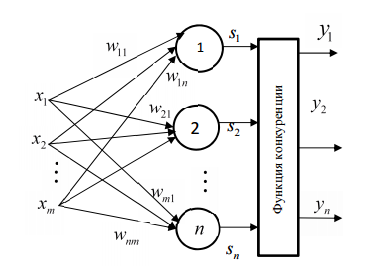
\includegraphics[width=0.8\textwidth]{network.png}
  \end{figure}
\end{frame}

\begin{frame}
  \frametitle{Геометрическая интерпретация}
  \begin{itemize}
    \item Каждому нейрону соответствует вектор размерности m из пространства
    входных данных.
    \item Для вектора x нейрон, который ближе всего по евклидову расстоянию,
    выдаст 1, остальные 0.
    \item
    \[
      \rho_{j}(x)^{2}=\|x-W_{j}\|^{2}=\|W_{j}\|^{2}-2\sum _{{i=1}}^{m}w_{{ji}}x_{i}+\|x\|^{2}
    \]
    \[
      j_{\max }={\rm {arg}}\max _{j}\left\{\sum _{i=1}^{m}w_{ji}x_{i}-{\frac {1}{2}}\|W_{j}\|^{2}\right\}
    \]
    $\rho_{j}(x)$ - расстояние до $j$-го нейрона. 
  
  \end{itemize}
\end{frame}

\begin{frame}
  \frametitle{Самоорганизующаяся карта Кохонена (Self-organizing map — SOM)}
  Нейронная сеть с обучением без учителя,
  выполняющая задачу визуализации и кластеризации.
\end{frame}

\begin{frame}
  \frametitle{Структура}
  Каждый нейрон состоит из двух векторов:
  \begin{itemize}
    \item вектор в пространстве входных данных (веса нейрона);
    \item вектор положения на карте(как правило, размерности 2).
  \end{itemize}
\end{frame}

\begin{frame}
  \frametitle{Нейроны образуют сетку}
    \begin{figure}
      \centering
      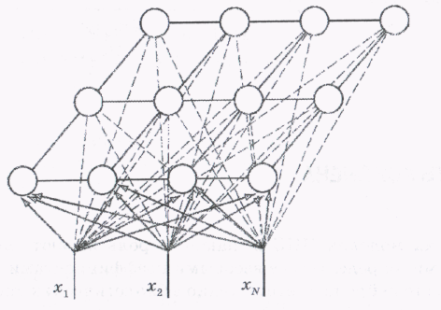
\includegraphics[width=0.7\textwidth]{structure.png}
    \end{figure}

\end{frame}

\begin{frame}
  \frametitle{Каждая ячейка - нейрон}
  \begin{figure}
    \centering
    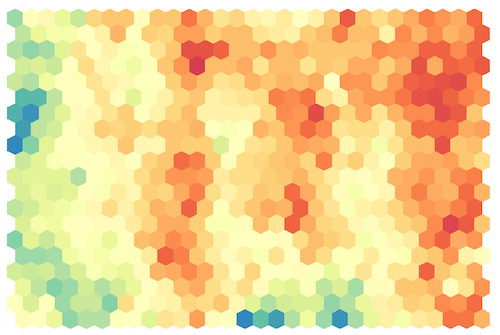
\includegraphics[width=0.8\textwidth]{every-cell-neuron.png}
  \end{figure}
\end{frame}

\begin{frame}
  \frametitle{Обучение}
  \begin{enumerate}
    \item инициализируем веса нейронов
    \item берём случайный вектор $D(t)$ из множества входных данных
    \item изменяем веса нейронов по формуле:
    \[
      W_v(s + 1)=W_v(s)+\theta(u, v, s) \cdot \alpha(s) \cdot (D(t) - W_v(s)),
    \]
    \item повторяем c шага 2, пока $s < k$
  \end{enumerate}

\end{frame}

\begin{frame}
  \frametitle{Веса нейронов приближаются к входным данным}
  \begin{figure}
    \centering
    \def\svgwidth{\columnwidth}
    \input{../img/Somtraining.pdf_tex}
  \end{figure}
\end{frame}

\begin{frame}
  \frametitle{U-matrix}
  \begin{itemize}
    \item Унифицированная матрица расстояний(unified distance matrix, U-matrix)
    - один из способов представления получившейся карты;
    \item Каждый нейрон раскрашиваем в зависимости от удалённости от него
    соседей.
  \end{itemize}
\end{frame}

\begin{frame}
  \frametitle{Пример U-matrix}
  \begin{figure}
    \centering
    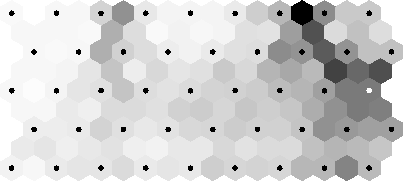
\includegraphics[width=0.8\textwidth]{u-matrix.png}
  \end{figure}
\end{frame}

\begin{frame}
  \frametitle{Другие виды представлений}
  \begin{itemize}
    \item Карта входов нейронов \\
    Для каждого входа рисуется своя карта, раскрашенная в соответствии со
    значением конкретного веса нейрона.
    \item Карта выходов нейронов \\
    На карту выходов нейронов проецируется взаимное расположение исследуемых
    входных данных.
    \item Специальные карты \\
    Это карта кластеров и карты, характеризующие их.
  \end{itemize}
\end{frame}

\begin{frame}
  \begin{figure}
    \centering
    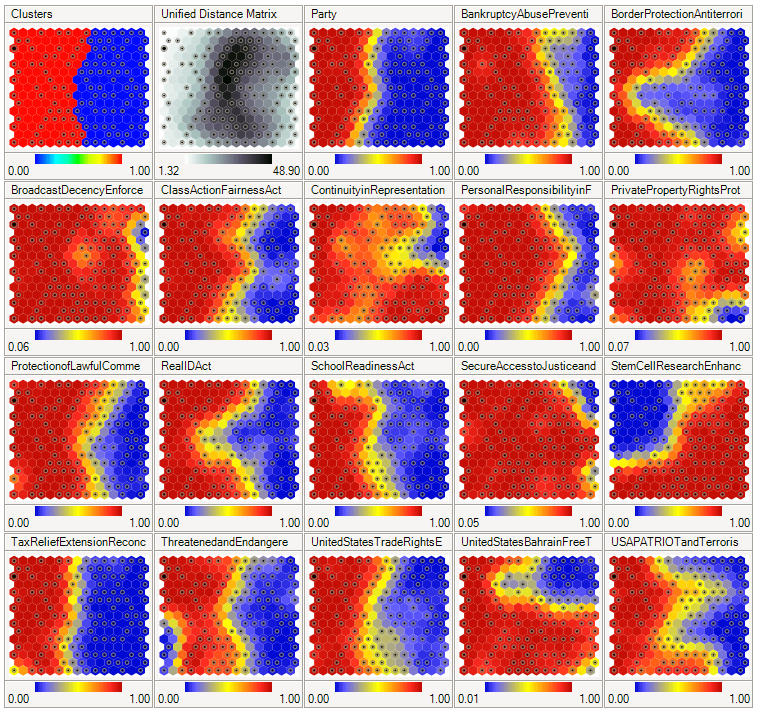
\includegraphics[width=0.65\textwidth]{congress.png}
  \end{figure}
\end{frame}

\begin{frame}
  \frametitle{Применение в искусстве}
  \begin{figure}
    \centering
    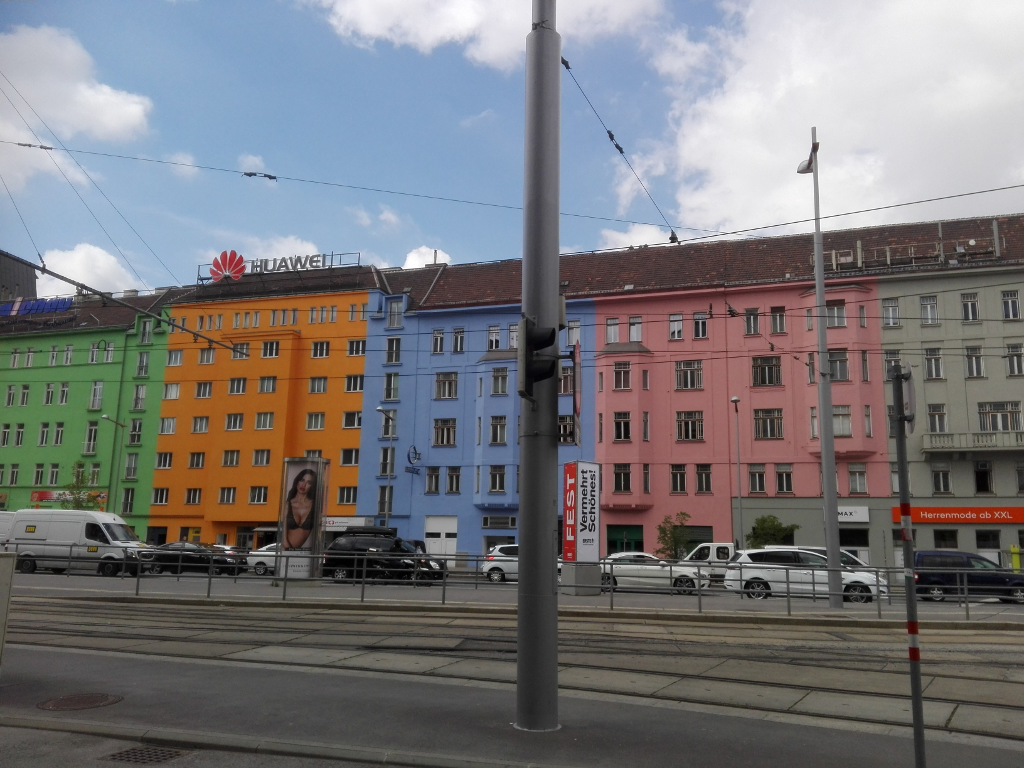
\includegraphics[width=0.75\textwidth]{street-before.png}
  \end{figure}
\end{frame}

\begin{frame}
  \frametitle{Применение в искусстве}
  \begin{figure}
    \centering
    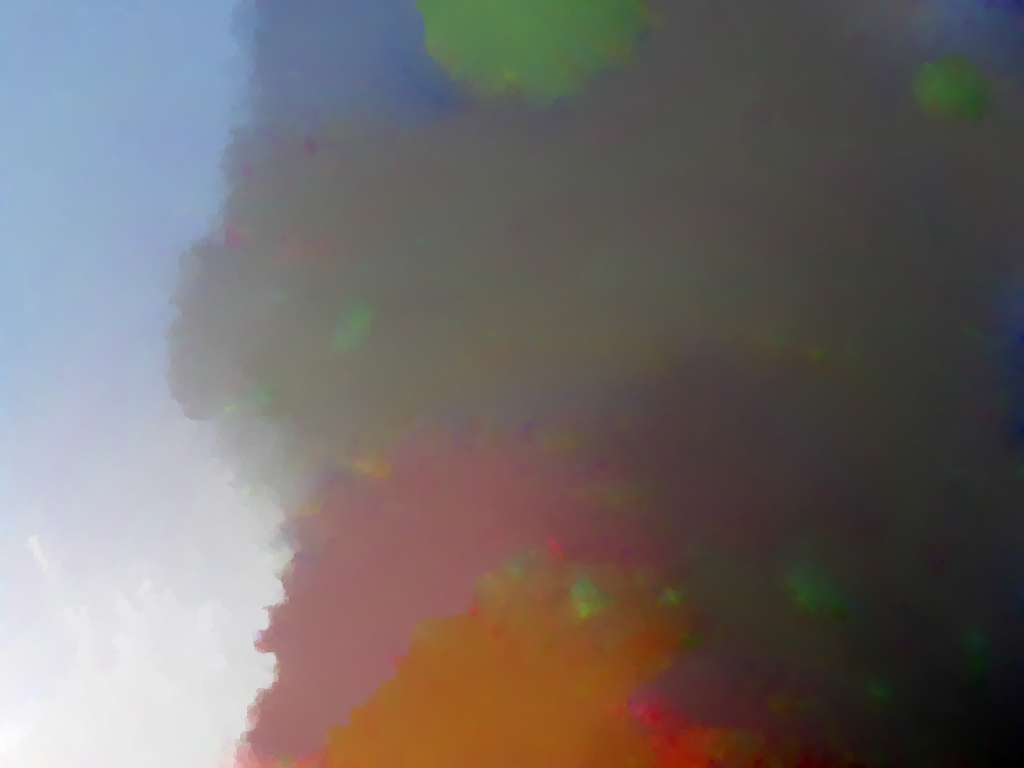
\includegraphics[width=0.75\textwidth]{street-after.png}
  \end{figure}
\end{frame}

\end{document}